



Al fine di valutare se la scelta della tecnologia SiC-CsI può soddisfare le esigenze di NUMEN è stata implementata una simulazione Monte Carlo sulla piattaforma GEANT4.
In questo capitolo vengono esposte le principali assunzioni e vengono presentati i risultati.



%Le simulazioni giocano un ruolo fondamentale nella fisica.

%In fisica, come in altre scienze, le simulazioni giocano un ruolo fondamentale, in quanto permettono di studiare la risposta di sistemi complessi tenendo sotto controllo alcuni dei suoi gradi di libertà.

\section{\iflanguage{italian}{Le simulazioni computerizzate e i metodi Monte Carlo}{Computer simulations and Monte-Carlo methods}}


In fisica, come in altre scienze, le simulazioni computerizzate giocano un ruolo fondamentale, in quanto permettono di affrontare lo studio di sistemi che sarebbero difficilmente trattabili utilizzando tecniche teoriche o sperimentali~``classiche'';
spesso, infatti, tali approcci possono presentare problematicità legate alla complessità del sistema, al tempo necessario per lo sviluppo e l'analisi, ai costi per la realizzazione di prototipi.
Introdotte negli anni Trenta grazie all'apporto di prestigiosi scienziati come von Neumann, Ulam e Fermi, il loro progresso è stato parallelo a quello dei computer, arrivando oggi ad essere uno strumento imprescindibile in molti esperimenti.
Esse forniscono una diversa prospettiva con cui guardare alla realtà, diventando in alcuni casi una base teorica da cui partire per l'interpretazione dei risultati sperimentali, oppure in altre situazioni producendo dati ``sperimentali'' con cui mettere al vaglio le teorie.


Tra i diversi metodi di simulazione computerizzata, particolare importanza hanno assunto i cosiddetti \emph{metodi Monte Carlo}~\cite{metropolis:jasa49}, il cui nome fu coniato da Metropolis ispirandosi al casinò omonimo.
%Tali metodi utilizzano la generazione di sequenze di numeri \emph{pseudo-casuali} per simulare le fluttuazioni statistiche di un sistema con un numero elevato di gradi di libertà, 
%laddove i numeri pseudo-casuali sono dei numeri prodotti in modo deterministico ma con proprietà statistiche simili a quelle dei numeri casuali.
%
Il numero di problemi che al giorno d'oggi vengono studiati utilizzando questa tecnica è enorme, annoverando campi di ricerca estremamente diversi, che vanno dalla fisica nucleare alla fisica medica, dalla meccanica statistica alla sociofisica, dall'economia alla biologia.
%Darne una definizione comprensiva di tutte le aree di interesse è un compito difficile e sostanzialmente inutile.
%
% ***** QUESTO NON ERA MALE
%Sebbene darne una definizione comprensiva di tutte le aree di interesse sia un compito difficile, in generale è possibile dire che i metodi Monte Carlo utilizzano la generazione di numeri casuali per simulare le fluttuazioni statistiche di un sistema con un numero elevato di gradi di libertà accoppiati.
%
%
Sebbene darne una definizione comprensiva di tutte le aree di interesse sia un compito difficile, in generale è possibile dire che i metodi Monte Carlo sono dei metodi numerici di risoluzione di equazioni o di calcolo di integrali basati sulla generazione di numeri casuali.
%I metodi Monte Carlo utilizzano la generazione di numeri casuali per simulare le fluttuazioni statistiche di un sistema con un numero elevato di gradi di libertà.
Il generico metodo si compone principalmente di quattro fasi:
\begin{itemize}
	\item generazione di una sequenza di numeri casuali;
	\item calcolo delle variabili di input sulla base della sequenza estratta;
	\item determinazione delle variabili di output utilizzando le variabili di input calcolate;
	\item ripetizione dei punti precedenti e analisi critica dei risultati.
\end{itemize}



%Dal momento che i metodi Monte Carlo dipendono fortemente dalla produzione veloce ed efficiente di flussi di numeri casuali, si preferisce generare le sequenze di numeri via software, piuttosto che leggerli da tavole ad hoc.
%Tuttavia, poiché tali algoritmi sono, in realtà, deterministici, 
%In realtà, dal momento che, per ragioni di velocità ed efficienza, tali sequenze sono prodotte via software, i numeri sono \emph{pseudo-casuali}
%Per risolvere un problema complesso è necessaria una sequenza molto grande di numeri casuali, i quali devono essere indipendenti fra loro.
Affinché il metodo si dimostri efficace, è essenziale che la sequenza di numeri sia quanto più possibile casuale.
Dunque, proprio la casualità con cui vengono prodotti tali numeri rappresenta il punto più delicato del metodo e, forse, il suo limite più grande; infatti, per ragioni di velocità ed efficienza i numeri vengono generati via software, invece di basarsi su processi fisici realmente casuali.
%Tuttavia, dal momento che tali algoritmi sono inevitabilmente deterministici, le sequenze di numeri sono, in realtà, \emph{pseudo-casuali}, ovvero presentano delle proprietà statistiche simili a quelle dei numeri casuali. 
Tuttavia, dal momento che tali algoritmi sono inevitabilmente deterministici, ogni numero della sequenza è univocamente calcolato a partire dal suo predecessore. 
Quindi, le sequenze di numeri sono, in realtà, \emph{pseudo-casuali}, ovvero, pur essendo deterministiche, presentano delle proprietà statistiche analoghe a quelle delle sequenze di numeri casuali. 
Per questo motivo, una successione di numeri pseudo-casuali non può avere elementi infinitamente diversi, in quanto, prima o poi, cominceranno a ripetersi.

Negli ultimi trent'anni l'importanza delle simulazioni basate su metodi Monte Carlo è cresciuta senza soluzione di continuità. 
%Uno dei motivi di tale successo deriva in quanto al crescere della complessità del problema tale tecnica risulta superiore rispetto agli approcci analitici in termini di tempo necessario per la 
%Uno dei motivi di tale successo deriva dalla maggiore efficacia di queste tecniche rispetto agli approcci analitici nella risoluzione di problemi caratterizzati da alta complessità;
%ad esempio, valutando l'efficacia di un metodo in termini del tempo necessario per risolvere un problema, al crescere della complessità risulta che tale tempo cresce più lentamente per i metodi Monte Carlo in confronto ai metodi analitici.
%come illustrato in Figura~\ref{fig:monte_carlo}, il tempo necessario 
%Uno dei motivi di tale successo deriva dalla grande efficacia di queste tecniche nella risoluzione di problemi altamente complessi;
Una delle ragioni di tale successo deriva dalla grande efficacia di queste tecniche nell'affrontare lo studio di sistemi con un numero elevato di gradi di libertà accoppiati; 
ad esempio, è possibile dimostrare che, al crescere della complessità del problema, i metodi Monte Carlo richiedono meno tempo per giungere alla soluzione rispetto alle tecniche analitiche o deterministiche, come mostrato in Figura~\ref{fig:monte_carlo}.


\begin{figure} [!t]
	\centering
	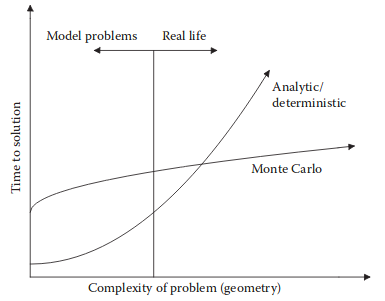
\includegraphics[scale=0.75]{Grafici/monte_carlo_vs_analytic2.png}
	\caption{Confronto fra il tempo necessario per la risoluzione di un problema con un metodo analitico-deterministico e con un metodo Monte Carlo, al variare della complessità del problema.} \label{fig:monte_carlo}
\end{figure}


%Nel campo della fisica, i metodi Monte Carlo sono spesso utilizzati per 
%Un notevole impulso allo sviluppo dei metodi Monte Carlo è provenuto dalla fisica delle alte energie, in cui l'elevata complessità degli apparati di rivelazione necessitava di uno strumento per decidere le specifiche in fase di progettazione.


%Un notevole impulso allo sviluppo dei metodi Monte Carlo è provenuto dalla fisica delle alte energie, in cui la crescente necessità di simulare complessi sistemi di rivelazione spingeva per la realizzazione di software sempre più performanti e robusti.
%
% ***** PRIMA AVEVO MESSO QUESTA
%Un notevole impulso allo sviluppo dei metodi Monte Carlo è provenuto dalla fisica delle alte energie, in cui si comprese che tali metodi offrivano la possibilità di seguire la traccia delle particelle e simulare le loro interazioni con la materia.
%
Un notevole impulso allo sviluppo dei metodi Monte Carlo è provenuto dalla fisica delle alte energie, in cui si comprese che tali metodi, offrendo la possibilità di seguire la traccia delle particelle e simulare le loro interazioni con la materia, potevano essere impiegati sia per la progettazione dei rivelatori sia per lo studio della loro risposta nelle condizioni sperimentali di interesse.
In questo contesto nacque il codice \emph{GEANT}, di cui nella sezione successiva si espongono le principali caratteristiche.





\section{\iflanguage{italian}{La piattaforma \textsc{Geant4}}{\textsc{Geant4} toolkit}}

%\section{\textsc{Geant4}}

La piattaforma GEANT, il cui nome deriva da \emph{GEometry ANd Tracking}, fu sviluppata nel 1974 al CERN di Ginevra allo scopo di simulare l'interazione di particelle elementari ad alta energia con i rivelatori.
%Questa prima versione consentiva di simulare il trasporto di un numero ristretto di particelle 
%In questa prima versione era possibile simulare soltanto un numero ristretto di particelle
In questa prima versione era possibile considerare soltanto un numero ristretto di particelle e forme geometriche semplici. 
Nel 1982 venne distribuito GEANT3, scritto in FORTRAN e nettamente potenziato rispetto al suo predecessore; infatti, si potevano simulare apparati sperimentali grandi e sofisticati e fasci di particelle molto intensi ed energetici.
Tuttavia, il codice presentava una struttura molto complessa, che rendeva difficile l'introduzione di nuove caratteristiche o la ricerca di errori.
%the simulation software geant4, which means \emph{geometry and tracking}, is a toolkit based on
%Fu così che si arrivò al 1998, anno dell'uscita dell'ultima versione del codice, chiamata \geant, interamente basata sul linguaggio C++.
%La crescente necessità di simulare complessi sistemi di rivelazione spingeva per la realizzazione di software sempre più performanti e robusti.
%
%%Fu così che nel 1998, grazie alla collaborazione di oltre 40 istituti internazionali, venne pubblicata l'ultima versione del codice, chiamata \geant.
D'altro canto, la crescente necessità di simulare complessi sistemi di rivelazione spingeva per la realizzazione di software sempre più performanti e robusti.
Fu così che nel 1998, grazie alla collaborazione di oltre 40~istituti internazionali, venne pubblicata l'ultima versione del codice, chiamata \geant.
Essa è interamente basata sul linguaggio C++, traendo vantaggio, dunque, da tutte le potenzialità offerte da una tecnologia orientata agli oggetti, come ad esempio la modularità e la compattezza.
% oppure il polimorfismo
%Il modo più corretto di definire \geant{} è \emph{toolkit}, ovvero ``cassetta per gli attrezzi'', in quanto comprende un insieme di librerie software che l'utente può selezionare a seconda delle proprie esigenze per creare un'applicazione specifica.

Oggi \geant{} consente di simulare l'interazione con la materia di tutte le particelle note, in un range energetico che va da pochi~eV fino ai~TeV.
%
%La sua notevole duttilità lo ha reso uno strumento 
Grazie alla sua notevole duttilità, sono innumerevoli gli esperimenti che si avvalgono di questo strumento e la sua area d'azione va dalla fisica delle alte energie, agli studi nucleari, alle applicazioni in campo medico, fino all'astrofisica.
Il codice è, inoltre, open-source e viene periodicamente aggiornato dalla collaborazione. 
Dal momento che la documentazione su \geant{} è ampia e dettagliata\footnote{Si veda, ad esempio, \url{www.geant4.cern.ch}}, nel prosieguo vengono presentati soltanto gli aspetti utili alla comprensione della simulazione svolta per questo lavoro di tesi.  



\subsection{\iflanguage{italian}{La struttura di \textsc{Geant4}}{\textsc{Geant4} structure}}

%Il modo più corretto di definire \geant{} è \emph{toolkit}, ovvero ``cassetta per gli attrezzi'', in quanto comprende un insieme di librerie software che l'utente può selezionare a seconda delle proprie esigenze per creare un'applicazione specifica.
Il modo più corretto di definire \geant{} è \emph{toolkit}, ovvero ``cassetta per gli attrezzi'', in quanto è costituito da un insieme di librerie software che, a seconda delle esigenze, possono essere selezionate per creare un'applicazione specifica.
L'utente deve, quindi, scrivere la sua applicazione, definendo tutti i parametri rilevanti: alcuni devono essere inseriti in modo obbligatorio, altri possono essere aggiunti facoltativamente.
%\geant{} offre numerose funzionalità:

Ogni simulazione si compone dei seguenti aspetti: 
\begin{itemize}
	\item la geometria del sistema e i materiali utilizzati, specificando forma, dimensione e posizione dei vari oggetti;
	\item la sorgente delle particelle, di cui si definisce la posizione, l'energia, la distribuzione angolare e tutte le altre caratteristiche rilevanti;
	\item i processi fisici di interazione per la modellizzazione  del comportamento delle particelle;
	\item il tracciamento delle particelle, che può essere calcolato anche passo dopo passo, consentendo di estrarre ad ogni step informazioni legate alla particella, come ad esempio energia e posizione;
	%\item la sensitività di un rivelatore e la sua risposta;
	\item la definizione di elementi sensibili, che simulano la risposta del rivelatore;
	\item la visualizzazione tridimensionale degli oggetti simulati e delle tracce delle particelle.
\end{itemize}


%Ciascuno degli aspetti elencati corrisponde ad una determinata \emph{classe} o \emph{categoria}, che, agendo in modo indipendente l'una dall'altra, danno al software una struttura modulare.

Gli aspetti elencati corrispondono nel toolkit a determinate \emph{classi} o \emph{categorie}, che, agendo in modo indipendente l'una dall'altra, danno al software una struttura modulare.
Esse sono state concepite per essere facilmente estendibili o modificabili dall'utente, seguendo la logica tipica dei linguaggi orientati agli oggetti.
%Di tutte le classi messe a disposizione, \geant{} richiede obbligatoriamente l'implementazione e l'istanziazione di tre, ovvero 
%\geant mette a disposizione un grande numero di classi, le quali sono state  concepite per essere facilmente estendibili o modificabili dall'utente, seguendo la logica tipica dei linguaggi orientati agli oggetti.
%L'implementazione e l'istanziazione di queste classi sono obbligatorie in tre casi, ovvero
%\geant{} mette a disposizione un grande numero di classi, ma per tre di loro l'implementazione e l'istanziazione sono obbligatorie.
\geant{} mette a disposizione un grande numero di classi, richiedendo obbligatoriamente l'implementazione e l'istanziazione per tre di loro: quella dedicata alla definizione della geometria e dei materiali; quella prevista per la definizione delle particelle, dei processi fisici e dei parametri di cut-off; quella rivolta alla generazione delle particelle primarie.





\clearpage


\section{\iflanguage{italian}{Gli aspetti principali della simulazione}{Simulation main aspects}}



\section{\iflanguage{italian}{I risultati}{Results}}


